\chapter{Enhancing Language Model}
\label{chapter:langModel}
%%===========================================================================%%
In this chapter we will look at several extensions to the baseline language
model.
%%
The first extension is to add an additional feature input channel to the
language model aimed at helping us effectively utilize the multiple new image
features proposed in Chapter~\ref{chapter:VisFeatChapter}.
%%
We then discuss an adaptation of the residual connections, recently proposed for
CNNs, to the LSTM language models.
%%
This allows us to effectively train deeper LSTM language models.
%%
Next we look at utilizing a hierarchical factorized decoder at the language
model output, in a bid to produce richer captions.
%%
Finally, a few ensembling techniques for combining multiple language models are
also presented.

\section{Additional Feature Inputs}
%%
The language model we use should be capable of simultaneously utilizing
different kinds of visual features presented in
Chapter~\ref{chapter:VisFeatChapter}.
%%
However, the baseline language model, presented in Chapter~\ref{chapter:baseline} has
only one input channel, shared between the word vectors and image features.
%%
Hence, in the baseline model the visual features are input to the network only
in the zeroth round of iteration.
%%
We refer to this input channel as the \emph{init} input to the LSTM network.
%%
This technique was also proposed in~\cite{Vinyals_2015_CVPR} as a solution to
prevent overfitting. 
%%
Therefore, the only way the baseline language model can utilize multiple visual
features is if they are fused into a single vector before presenting to the
language model.
%%
In our experiments, we have unfortunately found that performing simple feature
fusion, such as concatenating the two feature vectors, and using it as an input
in the baseline language model leads to inferior performance.
%%

To address this issue, another data input channel is introduced to the language
model proposed in this thesis.
%%
Furthermore, utilizing the new input channel, the visual features are made
available through the whole inference process.
%%
This requires adding a new input path to the LSTM cell which we refer to as the
\emph{persist} input.
%%
This is illustrated in figure~\ref{fig:proplstmlang}.
%%
Note that the \emph{persist} input plays the same role as $x(t)$ in
equations~(\ref{eqn:lstmstrt})--(\ref{eqn:lstmend}), but it has its own set of
input weights.
%%
For brevity, we will not repeat them here.
%%
Accordingly, the proposed framework computes the distribution
%%
\begin{equation}
p(w_t | w_{t-1},\cdots,w_0, I, P) = \text{softmax}(D y(t)) \;,
\end{equation}
%%
\noindent where $I$ and $P$ represent the \emph{init} and \emph{persist}
features respectively.
%%
Training is again done by minimizing the negative log likelihood cost function
as in the baseline model:
%%
\begin{align}
  %\label{eqCost}
  \mathcal{NL}(w_0,\cdots, w_{L-1} | I, P) = -\sum_{t=0}^{L-1} \log(p(w_t|w_{t-1},I,P)) \; .
\end{align}

%%
Having separate input matrices for \emph{init} and \emph{persist} features
allows the model to learn different functions from the word embeddings and the
visual features and in-turn makes the language model more powerful.
%%
We can also now input different visual features in the \emph{init} and
\emph{persist} paths thereby allowing the model to learn simultaneously from two
complimentary sources.

\begin{figure*}[t]
\begin{center}
  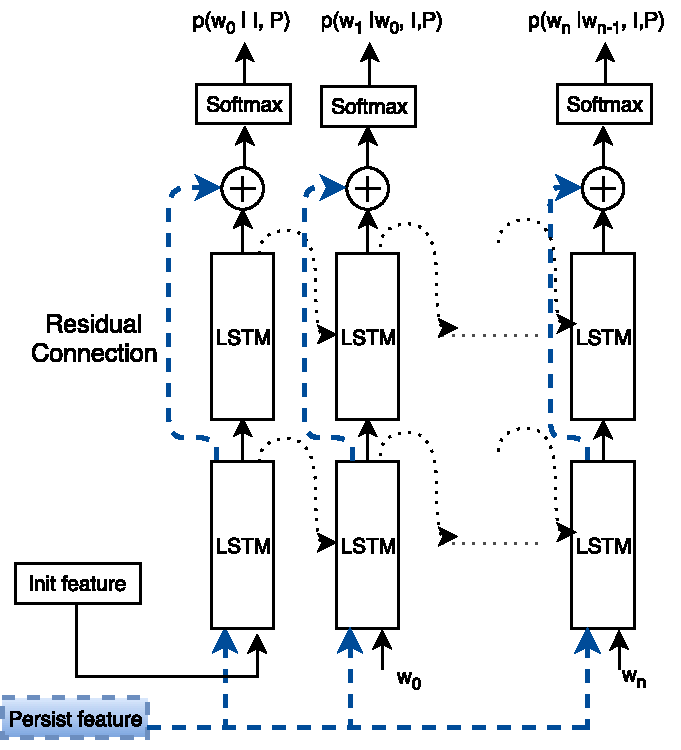
\includegraphics[width=0.7\linewidth]{images/MultilayerResidualLSTM.pdf}
\end{center}
\vspace*{-4mm}
\caption{The proposed language model architecture. The dashed blue lines
        highlight the changes proposed over the baseline. A two-layer LSTM with
residual connections is shown here.}
\label{fig:proplstmlang}
\end{figure*}

%%===========================================================================%%
\section{Deeper Models Using Residual Connections }
%% ---------------------------------------------------------------------------
Another extension we experiment with to improve the performance of our language
model is to add depth to the LSTM network used in it.
%%
Here, only the first LSTM layer receives the feature inputs directly and the
higher LSTM layers take their input $x(t)$ from the previous layer in the
network.
%%
The recurrent connections from a network's outputs back to its inputs exist only
within an LSTM layer and not across the layers.
%%
Softmax is applied at the output of the last LSTM layer only.
%%

Residual connections were recently proposed in~\cite{He2015} to be used in CNNs.
%%
The method consists of adding a fixed identity connection from the output of a
lower layer, $f_1(x)$, to the output the layer above it, $f_2(x)$.
%%
This alters the output after two layers from $f_2(f_1(x))$ to $f_1(x)+f_2(f_1(x))$.
%%
Now the second layer only needs to learn a residual function to push the
output of the first layer towards the desired output.
%%
If the first layer is already performing well, this makes the task of the second
layer much easier.
%%
This seemingly simple technique allowed to train much deeper CNNs~(almost three
times of the GoogLeNet) and achieve state-of-the-art performance on ImageNet
dataset in the image classification task~\cite{He2015}.

Inspired by this success, we adapt the method to our LSTM language model and
add residual connections between the LSTM layers. 
%%
These residual connections, shown in Figure~\ref{fig:proplstmlang}, greatly
improve the training convergence speed.
%%
We have also found out that the use of residual connections produces
significantly lower values for both the training cost function and the model
perplexity, as will be presented in Section~\ref{subsec:exptdepth}.

%%===========================================================================%%
\section{Hierarchical Decoder}
\label{sec:ClassFact}
Analyzing the erroneous outputs from the baseline language model, one category of
mistakes we often see are where the model misses the fine-grain
classification between two closely related objects.
%%
For example, we have noticed that a person's gender is often described wrongly.
%%
Similar uncertainty is also seen in telling apart various fruits and vegetables.
%%
This happens because these objects often occur in similar language contexts and
hence the context cannot help differentiate them.
%%
To correctly identify them, the LSTM generator needs to learn really fine-grained
object classification.
%%

In this thesis, it is hypothesized that the above problem is exacerbated by the
language model essentially having to do a $Z$-way classification at every
time-step, where $Z$ is the size of the vocabulary.
%%
When the size of the vocabulary is large, e.g.\@ on the COCO dataset the vocabulary
contains 8790 words, this $Z$-way classification is a hard problem.
%%
Additional complexity arises because the errors made in the $Z$-way
classification at any time-step affects all future predictions made during the
generation of that caption.

We attempt to address this problem by splitting the $Z$-way classification into
two smaller hierarchical classification problems.
%%
To do this, the language model vocabulary is first split into $Z^c$ classes and
each word in the vocabulary is assigned to one class. 
%%
Then the conditional probability of a word given the context can be factorized
into two parts as follows:
\begin{equation}
  \label{eq:class} 
  P(w_t | I,P, W^{t-1}) = P(c_t| I,P, W^{t-1}) P(w_t | c_t, I,P,W^{t-1}) \; ,
\end{equation}
\noindent where $c_t$ is the class of word $w_t$ and $W^{t-1}$ is sequence of words
seen up to time $t-1$, ($w_0\cdots w_{t-1}$).

This allows us to split the $Z$-way softmax at the LSTM output into two parts, a
$Z^c$-way softmax to predict the correct class and a $Z_w^c$-way softmax to
predict the correct word within this class.
%%
Here $Z_w^c$ is the number of words within the class $c$.
%%
This hierarchy allows the language model to learn separate decoders for each
class, possibly allowing it to learn more fine-grained classification.
%%
The hierarchical structure is also more amenable to adding new words to the
vocabulary.
%%
Adding a new word to a specific class already transfers the knowledge the model
has about the class to the word, and the model only needs to learn the
probability distribution of the new word within the class.

\subsection{Clustering Words to Classes}
The first step in implementing the hierarchical structure in the decoder is to
cluster words into different classes.
%%
There are two kinds of approaches to do this clustering in the literature.
%%
The first group of methods use knowledge bases such as WordNet to find similar
words and group them together.
%%
The second category of methods are completely data-driven and use just the
training data statistics to build the clusters.
%%
Here we will look at two different methods relying solely on the COCO training
data to cluster words into classes.

\subsubsection*{Brown Clustering}
A popular data-driven clustering algorithm is \emph{Brown clustering} proposed
in~\cite{BrownClust}.
%%
It is a hierarchical agglomerative clustering algorithm which produces a hierarchical
tree-like clusters of all the words in the vocabulary.
%%
To begin with, all the words in the vocabulary are assigned to individual leaf
nodes. 
%%
Then, starting from the leaf nodes, two nodes whose merging would reduce the
clustering cost function the most are combined into a single node.
%%
The clustering cost function is simply the perplexity assigned by a class based
bi-gram model to the training corpus. 
%%
In our case the training corpus consists of all the reference captions in the
training set.
%%
The clustering cost can be written as a function of the given cluster
assignment, $C(.)$, as 
\begin{equation}
  \label{eq:brown} 
        Quality(C) = \frac{1}{n} log \prod_{i=1}^{n} P(C(w_i)|C(w_{i-1})) P(w|C(w_i)) \; ,
\end{equation}
\noindent where $C(.)$ is the mapping which assigns words $w$ to their cluster
$C(w)$.

The process is terminated once the number of nodes have been reduced to the
desired number of clusters, $Z^c$.
%%
Although this method produces hierarchical clusters, one can ignore the
hierarchy and take all the classes in the final output as independent classes in
the language model. 
\subsubsection*{$K$-means Clustering}

$K$-means is a simple yet very effective clustering algorithm widely used on
high-dimensional vectorial data.
%%
The algorithm tries to partition the set of input data vectors into $K$ clusters
such that each data point belongs to the cluster whose mean is closest to
it.
%%
Usually, the Euclidean distance is used to measure distance between data points.
%%
One cannot, however, directly use the $K$-means method to cluster words as one
cannot measure the distance between words.
%%
Instead, the word-embeddings which are learnt in the language model can be used
to represent words as vectors in $d$-dimensional space.
%%
With this modification, the Euclidean distance between word embeddings can be
used as a measure of distance between the words and thus the $K$-means algorithm
can be utilized to find into $Z^c$ cluster centers in the word embedding space,
by setting $K=Z^c$.
%%
Once $Z^c$ cluster centers are obtained, each word is assigned to its closest
center and this partitioning is used in the language model.

\subsection{Factorizing LSTM Decoder Output}
In order to implement the hierarchical decoder in our LSTM language model, we
need to split the decoder matrix, $D$ into a set of $Z^c+1$ smaller matrices.
%%
This set contains one $D_{cls}$ matrix of size $h_{sz} \times Z^c$ which is
used to compute the class probability.
%%
Here, $h_{sz}$ is the hidden size of the LSTM layer in the language model.
%%
It also has K class specific matrices ${D^{1},D^{2}\cdots D^{Z^c}}$,
each of the size $h_{sz}\times Z_w^c$.
%%
Here $Z_w^c$ is the number of words in the class $c$.
%%
Consequently, computation performed to predict the word at time-step $t$ has two
stages, first to predict the right class of the word and then using the class
specific decoder matrix to predict the word within the class:
\begin{align}
        \label{eq:classLStmdecoder}
        P(c_{t}^{k}| I,P, W^{t-1}) &= \text{softmax}(D_{cls} y(t)) \\
        c_t &= \argmax_k\left(P(c_{t}^k| I,P, w^{t-1})\right) \\
        P(w_t | I,P, w^{t-1}) &= P(c_t| I,P, w^{t-1}) \cdot \text{softmax}(D^{c_t} y(t))
\end{align}

In theory this model should be faster since we only need to compute the
two smaller matrix multiplications instead of the one large one.
%%
However, due to bottlenecks in our implementation, this hierarchical decoder
runs slower than the single-stage decoder.
%%===========================================================================%%
\section{Ensembling Techniques}
%%----------------------------------%%
Using the many different image features and the LSTM language model
architectures we have discussed before, we can train a set of different language
models.
%%
When examining the pool of captions generated by such models for a set of
images, we have found out that different models tend to generate the best
captions for different kinds of images and videos.
%%
This indicates that ensembling these different generative models could be a good
idea.
%%
If one could evaluate the suitability of a given caption for a
given image, one could possibly pick out the best candidate from the pool and
achieve better results than with any single model.
%%
In this section we will examine two methods of evaluating the suitability
of a caption to the visual input and thus effectively ensembling multiple
language models.
%%

Concretely, given an input image or video feature, $V$, and a set of $p$
candidate captions, $C_p = \left\{S_1,S_2,\cdots, S_p\right\}$, generated by $m$
language models, $LM = \left\{lm_1,lm_2,\cdots, lm_m\right\}$, we wish to find
the evaluation function $E(S|V)$, such that $\argmax_{S_i} E(S_i|V)$ is
the most suitable caption for $V$ in the set $C_p$.
%%
The value of $p \leq (b\times m)$, with $p<(b\times m)$ when same captions are
generated by multiple models.
%%
Note that this evaluation function is different from using evaluation metrics to
evaluate a captioning system, as here we are assessing the captions without
using the ground truth. 
%%

The first method relies on the caption-generating language models themselves to
evaluate the candidates, while the second method involves training a separate
evaluator model to measure the similarity between the candidate captions and the
visual input.
%%
We will examine them in detail in the following subsections.

%%----------------------------------%%
\subsection{Combining Models with Mutual Evaluation}
\label{subsec:MutEval}

In this technique, we utilize the same language models which generated the
captions to also evaluate the captions.
%%
All the LSTM language models presented so far learn the conditional probability
distribution of the caption given the visual input, $P(S|V)$.
%%
We utilize this probability, $P(S|V)$, as a measure of the goodness of the
caption w.r.t the input, and then use it to rank the candidate captions.
%%
Considering only the probability assigned to a caption $S_i$ by the language
model which generated it, we could pick the caption with the highest probability
score as the best caption.
%%
We refer to this method as ``Self-Eval'' in rest of the thesis. 

Alternatively, one could also get the candidate captions evaluated by all the
other models in the ensemble.
%%
Thus one gets $m$ scores per caption, which can then be used to pick the best
candidate either using the ``max-mean'' method or the ``max-max'' method.
%%
In the ``max-mean'' case, the candidate with the highest mean of probability
scores is chosen as the best caption.
%%
In the case of the ``max-max'' method, the candidate with the highest maximum among
the $m$ probability scores is chosen as the best candidate:
\begin{eqnarray}
  \label{eq:cmme} 
  \text{max-mean:}& S_{best} &= \argmax_{S_j}\left(\frac{1}{m}\sum_{i=1}^{m}
  P_{lm_i}(S_j | V)\right) \; ,\\
  \text{max-max:}& S_{best} &= \argmax_{S_j} \left(\max_i P_{lm_i}(S_j |
  V)\right) \; ,
\end{eqnarray}
\noindent where $P_{lm_i}$ is the probability distribution learned by model
$lm_i$.

Since in this method models are evaluating each others' sentences, we refer to it
as ``Mutual-Eval''. 
%%
This method is also similar to the peer-review model used in academic
publishing, where researchers with expertise in related fields evaluate each
others' work.
%%
It works best when all the models in the ensemble are equally competitive, with
expertise in slightly different sub-domains of the dataset.

%%----------------------------------%%
\subsection{CNN Evaluator}
The language models we described for the evaluation of candidate captions in the
previous subsection are trained generatively.
%%
Thus they need to learn to model both the semantic and syntactic structures of a
sentence and their relation to the input image.
%%
In our experiments, we have noticed that these language models indeed are very
effective at learning syntactic structures of sentences, and grammatical
mistakes are rare in the generated captions.
%%
Most of the errors in the generated captions are of semantic nature, wherein the
models tend to get the objects or the relations between the objects wrong.
%%
This could be because similar syntactic structures repeat across a large number of
reference captions in the training dataset, but similar semantic relations
are found only in smaller parts of the dataset.
%%
This indicates that the evaluator function should mainly focus on
evaluating the semantic correctness of the candidate captions, and not worry
about nitty-gritties of syntactic correctness. 
%%
Thus, a generatively trained model will be suboptimal at this task and
discriminative training would be more suitable. 
%%

A solution to address this is to discriminatively train a new model whose task is to
pick out the best candidate from the candidate set, given an input image or
video.
%%
We refer to this as an evaluator network.
%%
The network takes as input one visual feature vector and an input sentence and
computes a similarity score between them. 
%%
The model is composed of a convolutional network to encode the sentences into a
sentence embedding, and a projection matrix which projects the visual feature
into the same space as the sentence embedding.
%%
The cosine similarity measure is used to evaluate the similarity between the
sentence embedding vector and the projected visual feature vector. 
%%

The convolutional network we use to encode sentences is based on the
paper~\cite{kim:2014:CNNsent}, where it is used for sentence sentiment
prediction.
%%
Figure~\ref{fig:CNNEval} shows the block diagram of our CNN-based evaluator.  
%%
Here, the input sentence is represented as a sequence of word vectors, which can
either be statically initialized with some standard word vector encodings, such
as GloVe~\cite{pennington2014glove} or word2vec~\cite{mikolov2013distributed},
or learned during the training phase.
%%
These word vectors are fed into a convolutional neural network which computes an
encoding of the sentence.

%%To compute the similarity between the image and the sentence encoding, the image
%%feature vector is first projected into same representation space using a
%%projection matrix.
%%%%
%%The similarity is then computed between the projected image vector and the
%%sentence encoding to give a match score between the input image and the
%%candidate sentence.

\begin{figure*}[t] 
  \centering
  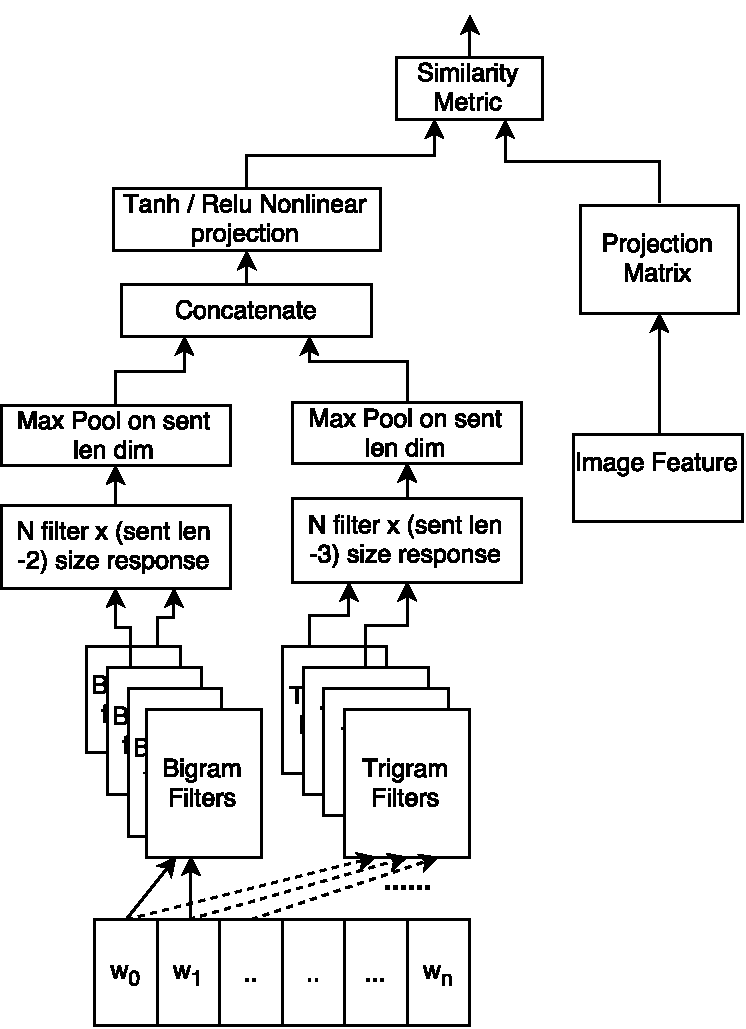
\includegraphics[width=0.6\textwidth]{./images/CnnEval.pdf} 
  \caption{CNN based evaluator network to compute the similarity between 
    an image and a caption.}
  \label{fig:CNNEval} 
\end{figure*}

% Convolutional network on sentences

The first layer in the CNN consists of convolutional filters of different sizes.  
%%
All the filters operate over the entire word vectors, but vary in the number of
words they cover, i.e., each filter is of the size $n \times
W_{\text{dim}}$. 
%%
Here, $n$ is the $n$-gram over which filter operates and $W_{dim}$ is the
dimensions of the word vector representation used in the CNN.
%%
For example, one can have filters operating over bigrams, trigrams, etc.
%%
Specifically, the CNN evaluator used in this work has filters with bigrams,
trigrams, 4-grams and 5-grams. 
%%
Additionally, $F_n$ number of filters of each $n$-gram type is used.
%%

The filter outputs are max-pooled, which reduces the filter response over entire
sentence into a single scalar, i.e., its maximum response. 
%%
We can therefore think of each filter as looking for a specific $n$-gram,
disregarding its location within the sentence.
%%
These pooled outputs are concatenated and then projected to the desired vector
size to produce the final sentence encoding.

%% --------------------------------------

\subsubsection{Training the Evaluator Network}

The evaluator network needs to be trained to assign a high score for the best
caption and lower scores for other captions.
%%
For each training set image or video $V$, the CNN evaluator scores the
corresponding ground truth caption, $S^+$, and $k$ negative samples, $S_i^-,
i=1,\ldots,k$, drawn randomly from the ground truth captions of other samples in
the training dataset.
%%
Now the training cost function $C$ is devised to maximize the score for the
positive sample and to minimize it for the negative samples. 
%%
This is achieved by applying a softmax on the scores of this batch (one positive
and $k$ negative samples) and maximizing the softmax score of the positive sample:
%%
\begin{align}
  \label{eq:cnnprob} 
  P(S^+|S^-,V) &= \frac{\exp(-f(S^+,V))}{\exp(-f(S^+,V)) +
           \sum\limits_i^k{\exp(-f(S_i^- ,V))}} \\
  C &= -\log P(S^+|S^-,V) \;.
\end{align}
%%
Equation~(\ref{eq:cnnprob}) shows this computation with $f(S,V)$ representing
the similarity metric between the sentence candidate $S$ and media $V$.
%%
In our current method, we use the cosine similarity between the two vectors for
the purpose of $f(S,V)$.

%% --------------------------------------

\subsubsection{Utilizing the Evaluator Network}

Once trained, the evaluator network can be utilized to compute the similarity
for a visual-input--caption pair.
%%
In this work, it is used to ensemble a set of language models.
%%
Concretely, every caption, $S_i$, in the candidate set, $C_p$, is paired with
the visual input and is fed to the evaluator network. 
%%
This gives us $p$ similarity scores $(E_{cnn}(S_0,V),\cdots,E_{cnn}(S_p,V))$,
one for each candidate caption, $S_i$.
%%
The candidate with the highest similarity is chosen as the output caption from
the ensemble for the visual input.

\begin{equation}
        S_{cnn} = \argmax_{S_i} E_{cnn}(S_i,V)\\
\end{equation}
%% ===========================================================================
